\documentclass{article}
\usepackage{arxiv}
\usepackage[utf8x]{inputenc}
\usepackage[english, russian]{babel}
\usepackage[T2A, T1]{fontenc}
\usepackage{url}
\usepackage{booktabs}
\usepackage{amsfonts}
\usepackage{nicefrac}
\usepackage{microtype}
\usepackage{lipsum}
\usepackage{graphicx}
\usepackage{natbib}
\usepackage{doi}
\usepackage{amsmath,amsfonts,amssymb,amsthm,mathtools}
\DeclareMathOperator*{\argmax}{\arg\!\max}
\DeclareMathOperator*{\argmin}{\arg\!\min}



\title{Ускорение семплирования из диффузионных моделей с использованием состязательных сетей}

\author{Охотников Н. В.\\
	\texttt{okhotnikov.nv@phystech.edu} \\
	\And
    Исаченко Р.В. \\
	\texttt{isa-ro@yandex.ru} \\
}
\date{}

\renewcommand{\shorttitle}{\textit{arXiv} Template}

%%% Add PDF metadata to help others organize their library
%%% Once the PDF is generated, you can check the metadata with
%%% $ pdfinfo template.pdf
\hypersetup{
pdftitle={A template for the arxiv style},
pdfsubject={q-bio.NC, q-bio.QM},
pdfauthor={Охотников Н.В., Исаченко Р.В.},
}
\begin{document}
\maketitle
\begin{abstract}
	В последние годы широкое распространение получили диффузионные генеративные модели, показывающие высокое качество получаемых семплов и хорошее покрытие исходного распределения. Главный их недостаток -- скорость семлирования: для получения одного объекта требуется от сотен до тысяч итераций. Активно исследуются способы ускорения этого процесса. В работе анализируется один из таких способов -- использование состязательных моделей для сокращения числа шагов, необходимых для получения семпла. Экспериментально исследуются влияние гиперпараметров представленной ранее модели Denoising Diffusion GAN \cite{https://doi.org/10.48550/arxiv.2112.07804} на скорость генерации, а также качество и разнообразие получаемых семплов. Рассматриваются альтернативные варианты задания сложного распределения в обратном диффузионном процессе.
\end{abstract}

\section{Введение}
 После того, как была представлена Denoising Diffusion Probabilistic Models (DDPM) \cite{https://doi.org/10.48550/arxiv.2006.11239} модели на ее основе становились все популярней, показывая лучшее или сравнимое со state-of-the-art состязательными сетями \cite{https://doi.org/10.48550/arxiv.1812.04948} качество генерации\cite{https://doi.org/10.48550/arxiv.2105.05233}, при значительно более простом процессе обучения и более широком покрытии исходного распределения. Несмотря на это, использование диффузионных моделей на практике часто слишком дорого, ввиду необходимости запуска сети до 2000 раз для генерации каждого семпла. Предлагались различные способы ускорения этого процесса \cite{https://doi.org/10.48550/arxiv.2102.09672}, многие из которых обощены в FastDDPM \cite{https://doi.org/10.48550/arxiv.2106.00132}, но большинство из них все еще требуют многих десятков итераций и не позволяют приблизиться к состязательным сетям по скорости генерации. В данной работе исследуется проблема дальнейшего ускорения семплирования.
 
 Основное предположение для большинства диффузионных моделей -- нормальность условного распределения следующего шага по предыдущему в обратном процессе. Это достигается лишь в приближении бесконечно малых во времени шагов, а значит на практике требует достаточного большого количества итераций. Существуют различные способы обойти это предположение и апроксимировать распределение сложными мультимодальными, один из них -- использовать GAN модели на каждом шаге обратного диффузного процесса. В одной из работ уже была представлена модель Denoising Diffusion GAN, реализовавшая эту идею. Подобный подход позволяет снизить необходимое количество шагов до нескольких единиц и добиться ускорения семплирования на 2 порядка в сравнении с оригинальной DDPM. В работе попробуем на эксперименте возпроизвести этот результат и исследовать другие возможности приближения сложными мультимодальными распределениями при семплировании из диффузионных моделей с приростом скорости и без потери качества.
 
 \section{Аппроксимация обратного диффузионного процесса мультимодальными распределениями}
 \subsection{Дифузионные модели}
 В стандартных дифузионных моделях \cite{https://doi.org/10.48550/arxiv.1503.03585, https://doi.org/10.48550/arxiv.2006.11239} рассматриваются прямой и обратный диффузионные процессы. Модель получает на вход сэмпл из исходного распределения $x_0\sim q(x)$ и в течение $T$ шагов создает зашумленные его версии $x_1\dots x_T$ по следующему правилу:
 \begin{equation}
 	q(x_t|x_{t-1}) = \mathcal{N}(x_t; \sqrt{1-\beta_t}x_{t-1}, \beta_t I)
 \end{equation}
Где $\{\beta_t \in (0, 1)\}_{t=1}^T$. Откуда принимая $\alpha_t = 1 - \beta_t,~~\overline{\alpha_t} = \prod_{i=1}^t \alpha_i$:
 \begin{equation}
	q(x_t|x_0) = \mathcal{N}(x_t; \sqrt{\overline{\alpha_t}}x_0, (1-\overline{\alpha_t})I)
\end{equation}

При достаточно больших $T$ со сколько угодно большой точностью $x_T\sim \mathcal{N}(0,I)$. Таким образом, прямой диффузионный процесс за большое число шагов, добавляя на каждом некоторый нормальный шум, сводит сэмпл из исходного распределения к сэмплу из стандартного нормального. 

Пусть $X = (x_0^1\dots x_0^n)\sim p_0(x)$ -- обучающая выборка, т.е. некоторые семплы из распределения, объекты которого модель должна научиться генерировать. $p(x_1\dots x_T) = p_\theta(x_T)p_\theta(x_{T-1}|x_T)\dots p_\theta(x_0|x_1)$ -- совместное распределение генерируемых на каждом шаге обратного процесса объектов. Тогда для построения обратного процесса воспользуемся методом максимального правдоподобия:
 \begin{equation}
	\theta =\argmax\limits_{\theta} p(X|\theta) = \argmax\limits_{\theta} \sum\limits_{i=1}^n \log{p(x_0^i|\theta)}
\end{equation}

 \begin{equation}	
	 \sum\limits_{i=1}^n \log{p(x_0^i|\theta)}\geqslant \sum\limits_{i=1}^n \mathcal{L}(\theta, q;x^i_0) = \sum\limits_{i=1}^n\int q(x_1\dots x_T)\log{ \frac{p(x_0^i,x_1\dots x_T)}{q(x_1\dots x_t|x_0^i)}}dx_1\dots x_T
\end{equation}
 Неравенство обосновано в \cite{https://doi.org/10.48550/arxiv.1312.6114}. Подставляя в правую часть известные из прямого процесса распределения и пользуясь формулой Байеса получаем, что для максимизации правой части требуется (см. \cite{https://doi.org/10.48550/arxiv.2006.11239}) минимизировать следующее выражение:
 \begin{equation}
 	 	\label{KL_loss}
	\sum\limits_{t=1}^n \mathbb{E}_{x_1\dots x_T} KL\left(q(x_{t-1}|x_t, x_0)~||~p_\theta(x_{t-1}|x_t)  \right)
\end{equation}
Для стандартной диффузионной модели после этого шага $p_\theta(x_{t-1}|x_t)$ принимается нормальным, что очевидно из теоремы Байеса в приближении малости шага, тогда KL-дивергенция существенно упрощается и после правильной параметризации $p_\theta(x_{t-1}|x_T)$ получаем итоговое выражение, которое оптимизируется в модели:
 \begin{equation}
	L(\theta) =  \sum\limits_{i=1}^n \sum\limits_{t=2}^n \frac{\beta^2}{2\overline{\beta_t} (1-\beta)(1-\overline{\alpha_t})} ||\varepsilon - \widehat{\varepsilon_\theta}(x_t^i, t)||^2\longrightarrow\min\limits_\theta
\end{equation}
где 
 \begin{equation*}
	\overline{\beta_t} = \frac{1-\overline{\alpha_{t-1}}}{1 - \overline{\alpha_t}}, ~~~~~~~~ \widehat{\varepsilon_\theta}(x_t^i, t) = \frac{x_t^i - \sqrt{\overline\alpha_t} x_0^i}{\sqrt{1-\overline\alpha_t}}
\end{equation*}

 \subsection{Мультимодальные распределения}
Итак, мы показали, что требование к большому количеству итераций в диффузионных моделях вытекает из предположения нормальности $p_\theta(x_{t-1}|x_t)$, необходимого для подсчета $KL$-дивергенции. Однако, это распределение также может быть проинтерпретировано 
как $p_\theta(x_{t-1}|x_t) = q(x_{t-1}|x_t,x_0 = f_\theta(x_t, t))$, т.е. как предсказание $x_0$ некоторой моделью, зависящей от времени и последующее зашумление его до семпла из $q(x_{t-1}|x_t,x_0)$ с помощью известных из прямого прохода переходов. Таким образом, если уметь аппроксимировать некоторое сложное мультимодальное распределение (одному зашумленному семплу соответствует целое множество из исходного распределения), то можно достичь поставленной цели -- значительно сократить количество итераций обратного прохода. 
\subsection{DDGAN}
Одним из возможных подходов для этого является использование состязательных сетей. В таком случае обратный процесс устроен следующим образом: для каждого времени $t$ из объектов $\{x_t^i\}$с помощью генератора получаем сэмплы $\{x_0^i\}$ из исходного распределения, последовательно добавляя шум получаем $x_{t-1}^i$, и применяем дискриминатор к парам из $x_{t-1}^i$ и истинных зашумленных объектов из прямого прохода $\{\widehat{x_t^i}\}$, который обучается определять, являются ли $x_{t-1}^i$ правдоподобными "расшумленными" версиями $\{\widehat{x_t^i}\}$. 

Подставляя в \ref{KL_loss} вместо $KL$-дивергенции метрику Васерштейна, дивергенцию Йенсена-Шеннона, f-дивергенцию и другие функции, использующиеся в различных подходах к обучению GAN моделей \cite{https://doi.org/10.48550/arxiv.1406.2661, 
		https://doi.org/10.48550/arxiv.1701.07875,
		https://doi.org/10.48550/arxiv.1606.00709,
		https://doi.org/10.48550/arxiv.2010.08029} 
как $D_{adv}$
получаем следующую задачу минимизации:
 \begin{equation}
	\min\limits_\theta\sum\limits_{t\geqslant 1}^n \mathbb{E}_{q(x_t)}[ D_{adv}\left(q(x_{t-1}|x_t, x_0)~||~p_\theta(x_{t-1}|x_t)  \right)]
\end{equation}
Зададим дискриминатор от параметров $\varphi$ как $D_\varphi(x_{t-1}, x_t, t)$, будем тренировать его на минимизацию следующего выражения:
 \begin{equation}
	\min\limits_\varphi\sum\limits_{t\geqslant 1}^n \mathbb{E}_{q(x_t)}[\mathbb{E}_{q(x_{t-1}|x_t)}[-\log{(D_\varphi(x_{t-1, x_t, t}))}] + \mathbb{E}_{p_\theta(x_{t-1}|x_t)}[-\log{(1 - D_\varphi(x_{t-1, x_t, t}))}]]
\end{equation}

С известным дискриминатором тренируем генератор на максимизацию:
 \begin{equation}
	\max\limits_\theta\sum\limits_{t\geqslant 1}^n \mathbb{E}_{q(x_t)}\mathbb{E}_{q(x_{t-1}|x_t)}[\log{(D_\varphi(x_{t-1, x_t, t}))}]
\end{equation}
Причем параметризуем целевое распределение следующим образом:
 \begin{equation}
	p_\theta(x_{t-1}|x_t) := \int p_\theta(x_0|x_t)q(x_{t-1}|x_t, x_0)dx_0 =\int p(z)q(x_{t-1}|x_t, x_0 = G_\theta(x_t, z, t))dz
\end{equation}
где $p_\theta(x_0|x_t)$ -- неявное распределение порождаемое генератором $G_\theta(x_t, zk, t):\mathbb{R}^N\times\mathbb{R}^L\mathbb{R}\to \mathbb{R}^N$, прогнозирующим $x_0$ по $x_t$ и свободной нормально распределенной переменной $z\sim p(z) := \mathcal{N}(z; 0, I)$. Введение такой случайной переменной и позволяет восстанавливаемому распределению стать сложным мультимодальным.

 \section{Вычислительный эксперимент}
Целью эксперимента является анализ влияния количества шагов обратного диффузного процесса на качество и скорость семплирования для различных способов ускорения. В качестве метрики качества используем FID-score \cite{https://doi.org/10.48550/arxiv.1706.08500}, тестируем все рассматриваемые модели на датасете FashionMNIST. 


\subsection{Диффузионная модель}
В качестве базового эксперимента, обучаем простую диффузионную модель аналогично \cite{https://doi.org/10.48550/arxiv.2006.11239}. Для различного количества шагов T обратного диффузионного процесса считаем FID. Полученная зависимость изображена ниже.

\newpage

\begin{figure}[h]
	\centering{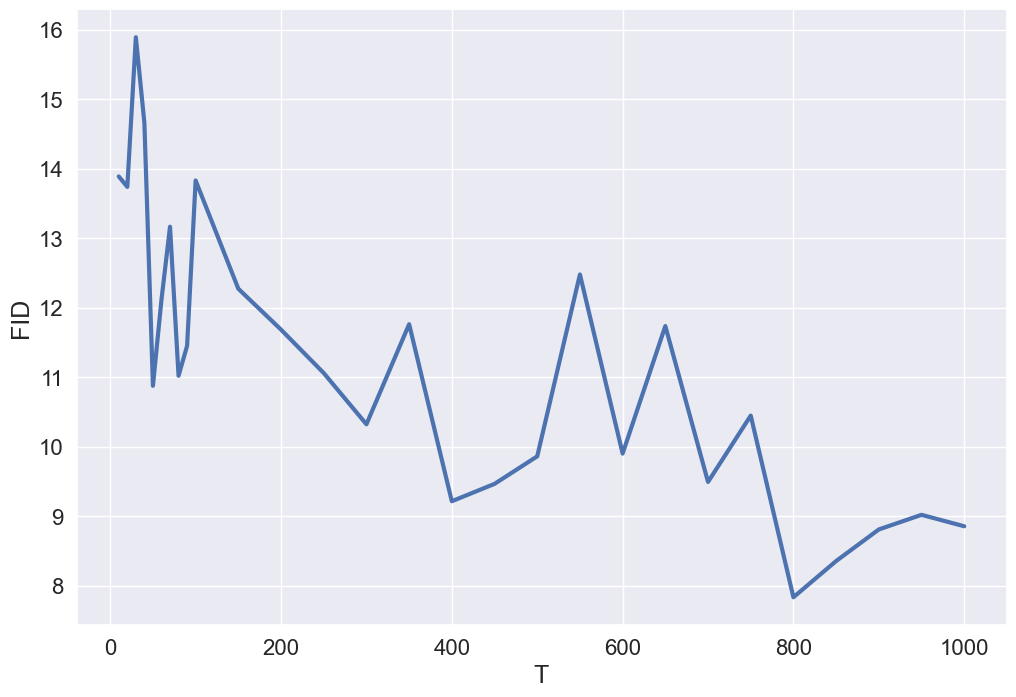
\includegraphics[scale = 0.4]{../code/DDPM_FID_FMNIST.png}}
	\caption{Зависимость FID от количества шагов}
\end{figure}

Несмотря на некоторые колебания, вызванные, вероятно, недостаточным числом тестовых семплов на каждой итерации, FID, как и ожидалось, падает с увеличением T.

\subsection{DDGAN}
...




\bibliographystyle{plain}
\bibliography{references}




\end{document}